\begin{figure}[!htb]
    \centering
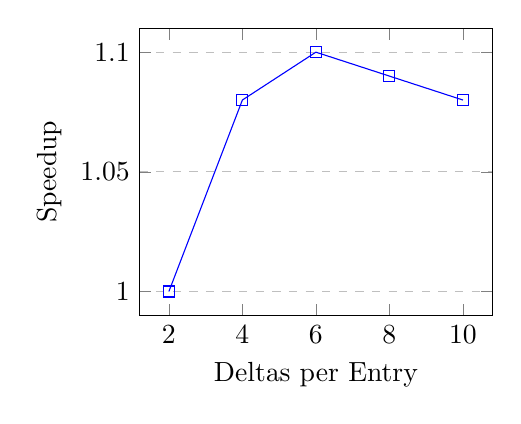
\begin{tikzpicture}
\begin{axis}[
    xlabel={Deltas per Entry},
    ylabel={Speedup},
    %xtick={0,1 ,2, 4, 8, 16},
    %ytick={0,0.5,1,1.5, 2},
    %nodes near coords,
    %nodes near coords align={vertical},
    legend pos=south east,
    ymajorgrids=true,
    grid style=dashed,
    width=\textwidth/2,
]
%DCPT
\addplot[
    color=blue,
    mark=square,
    ]
    coordinates {
    (2,1.00)(4,1.08)(6,1.1)(8,1.09)(10,1.08)
    };
    
    %\legend{DCPT, No Prefetch}
    
\end{axis}
\end{tikzpicture}
    \caption{Speedup of the DCPT algorithm with different amounts of deltas in each entry.}
    \label{fig:deltaEntries}
\end{figure}